\documentclass[tikz,border=8pt]{standalone}
\usepackage[scaled=0.95]{helvet}
\renewcommand{\familydefault}{\sfdefault}
\usepackage[europeanresistors,americanvoltages]{circuitikz}
\usepackage{amsmath}
\definecolor{TEJNavy}{HTML}{1E2B55}
\definecolor{TEJBlue}{HTML}{1769AA}
\definecolor{TEJOrange}{HTML}{E97828}
\begin{document}
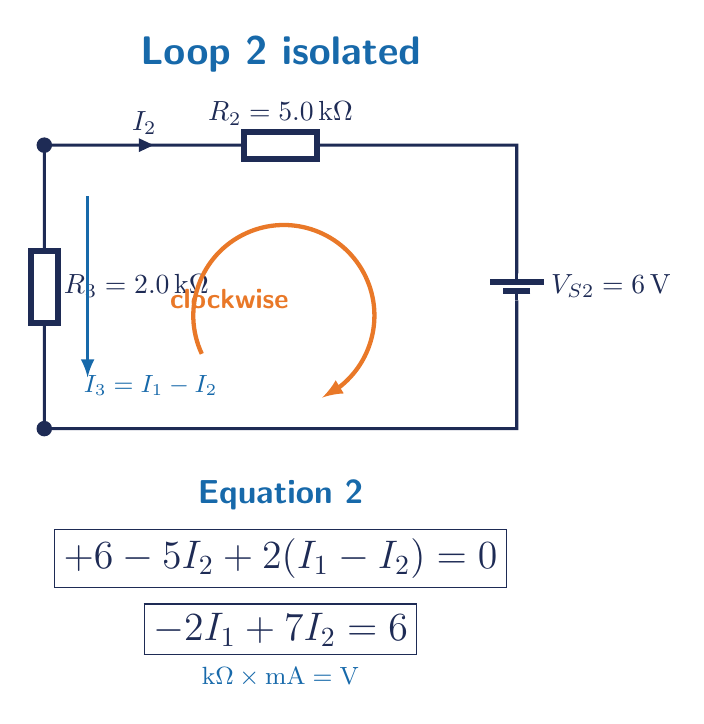
\begin{tikzpicture}[line width=1.1pt,draw=TEJNavy,text=TEJNavy,>=latex]
  \ctikzset{bipoles/length=1.15cm}
  \node[font=\bfseries\Large,text=TEJBlue] at (3.2,5.25)
    {Loop 2 isolated};

  \draw (0.2,4.1)
    to[R,l^={$R_2=5.0\,\mathrm{k}\Omega$},i>^={$I_2$}] (6.2,4.1)
    to[battery1,l^={$V_{S2}=6\,\mathrm{V}$}] (6.2,0.5)
    -- (0.2,0.5)
    to[R,l_={$R_3=2.0\,\mathrm{k}\Omega$}] (0.2,4.1);
  \fill[TEJNavy] (0.2,4.1) circle (2.8pt);
  \fill[TEJNavy] (0.2,0.5) circle (2.8pt);

  \draw[->,TEJOrange,line width=1.55pt]
    (2.2,1.45) arc[start angle=205,end angle=-65,radius=1.15cm];
  \node[font=\bfseries,text=TEJOrange] at (2.55,2.15) {clockwise};
  \draw[->,TEJBlue,line width=1.25pt] (0.75,3.45) -- (0.75,1.15);
  \node[font=\small,text=TEJBlue] at (1.55,1.05) {$I_3=I_1-I_2$};

  \node[font=\bfseries\large,text=TEJBlue] at (3.2,-0.35)
    {Equation 2};
  \node[font=\Large] at (3.2,-1.15)
    {$\boxed{+6-5I_2+2(I_1-I_2)=0}$};
  \node[font=\Large] at (3.2,-2.05)
    {$\boxed{-2I_1+7I_2=6}$};
  \node[font=\small,text=TEJBlue] at (3.2,-2.65)
    {$\mathrm{k\Omega}\times\mathrm{mA}=\mathrm{V}$};
\end{tikzpicture}
\end{document}
